\chapter{云计算关键技术}

\section{虚拟化}

\begin{definition}[虚拟化]
    通过该技术将一台计算机虚拟为多台逻辑计算机。 在一台计算机上同时运行多个逻辑计算机,每个逻辑计算机可运行不同的操作系统,并且应用程序都可以在相互独立的空间内运行而互不影响,从而显著提高计算机的工作效率。 
\end{definition}

\begin{example}[Amazon开启虚拟机]
    选择ami(guest OS image):支持的virtualization type (\term{paravirtual} 半虚拟化 $\rightarrow$ 性能不一致)
\end{example}

\begin{figure}
    \centering
    \begin{subfigure}[b]{0.3 \textwidth}
        \centering
        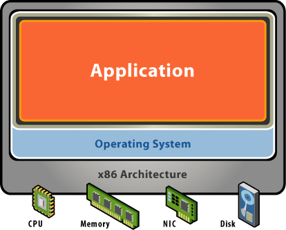
\includegraphics[width=\textwidth]{cloud-pc-architecture.png}
    \end{subfigure}
    \begin{subfigure}[b]{0.3 \textwidth}
        \centering
        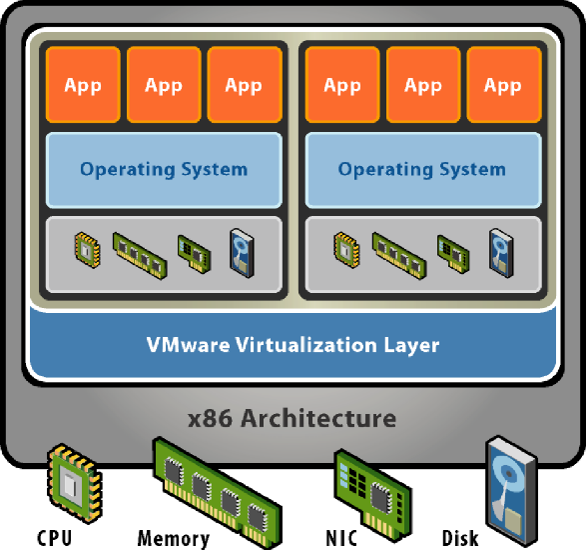
\includegraphics[width=\textwidth]{cloud-vmware-architecture.png}
    \end{subfigure}
\end{figure}

\begin{definition}[Host Machine]
    物理机
\end{definition}

\begin{definition}[Host OS]
    运行在物理机之上的OS
\end{definition}

\begin{definition}[Hypervisor, Virtual Machine Monitor (VMM)]
    虚拟机监控器
\end{definition}

\begin{definition}[Virtual Machine]
    虚拟出来的虚拟机
\end{definition}

\begin{definition}[Guest OS]
    运行在虚拟机之上的OS
\end{definition}

假如一个核分给2个虚拟机,则平台,OS需要分时切换。️ 网络的虚拟化隔离难以实现,因此虚拟化机网络性能不稳定, 虚拟机的网络转发到物理机的网络中。

虚拟化特点:

\begin{itemize}
    \item 分区: 在单一物理服务器上同时运行多个虚拟机
    \item 隔离: 在同一服务器上的虚拟机相互隔离
    \item 封装: 整个虚拟机都保存在文件中,而且可以通过移动和复制这些文件的方式来移动和复制该虚拟机
\end{itemize}

虚拟机上读取数据? 

硬件磁盘挂载在硬件上 guest OS转换请求到hypervisor$\rightarrow$ OS$\rightarrow$ 硬件以隔离不同虚拟机,overhead大

\subsection{从虚拟平台角度划分的分类}

\subsubsection{全虚拟化}

\begin{definition}[全虚拟化]
    虚拟的操作系统,与底层的硬件完全隔离,由中间的Hypervisor层转化。 
    
    典型的代表有Vmware WorkStation, Microsoft Virtrual Server. 
\end{definition}

\begin{definition}[KVM]
    KVM (for Kernel-based Virtual Machine) is a full virtualization solution for Linux on x86 hardware containing virtualization extensions (Intel VT or AMD-V). It consists of a loadable kernel module, kvm.ko, that provides the core virtualization infrastructure and a processor specific module, kvm-intel.ko or kvm-amd.ko
\end{definition}

完全隔离,由hypervisor层转换 

VMware workstation:速度减慢,性能瓶颈,隔离更好

\subsubsection{半虚拟化}

\begin{definition}[半虚拟化]
    虚拟机的操作系统当中加入特定的虚拟化指令,可以\textbf{直接通过Hypervisor调用硬件资源},免除了Hypervisor层转换指令的开销。 
    
    典型代表有Xen, Hyper-V
\end{definition}

使得OS和虚拟化层协同工作,减轻2层OS的负担,但是需对OS进行改动,OS知道正处于虚拟化环境中,开销减小

xen(也逐渐支持全虚拟化,以提升通用性)

\begin{definition}[Xen]
    The Xen Project community develops an open-source type-1 or bare-metal hypervisor, which makes it possible to run many instances of an operating system or indeed different operating systems in parallel on a single machine (or host). The project develops the only type-1 hypervisor that is available as open source. The hypervisor is used as the basis for a number of different commercial and open source applications, such as server virtualization, Infrastructure as a Service (IaaS), desktop virtualization, security applications, embedded and hardware appliances, and automotive. It enables users to increase server utilization, consolidate server farms, reduce complexity, and decrease total cost of ownership.
\end{definition}

\subsection{从虚拟化的层次划分}

\subsubsection{软件辅助的虚拟化技术}

\begin{definition}[软件辅助的虚拟化技术]
    通过软件的方法,让客户机的特权指令陷入异常,从而触发宿主机进行虚拟化。 如Hyper-V等。 
\end{definition}

\begin{definition}[Hyper-V]
    Hyper-V specifically provides hardware virtualization. That means each virtual machine runs on virtual hardware. Hyper-V lets you create virtual hard drives, virtual switches, and a number of other virtual devices all of which can be added to virtual machines
\end{definition}

\subsubsection{硬件支持的虚拟化技术}

\begin{definition}[硬件支持的虚拟化技术]
    在X86处理系统架构中加入新的指令机以及运行模式完成虚拟化操作,进而对硬件资源进行直接调用,进行虚拟化。 如AMD-V等。 
\end{definition}

\subsection{从虚拟化的实现结构划分}

\subsubsection{基于操作系统的虚拟化}
\begin{definition}[基于操作系统的虚拟化]
    在一个已存在的操作系统上安装虚拟化软件

    特点:
    
    \begin{itemize}
        \item 简单、易于实现
        \item 安装和运行虚拟化程序依赖于主机操作系统对设备的支持
        \item 有两层OS,管理开销较大,性能损耗大
        \item 虚拟机对各种物理设备的调用,都通过虚拟化层和宿主机的OS一起协调才能完成
    \end{itemize}

    例子:Vmware Workstation和VirtualBox等
\end{definition}

2层OS,易于实现,开销较大,需要管理层OS层转换请求 

如VMware

\subsubsection{基于硬件的虚拟化}

\begin{definition}[基于硬件的虚拟化]
    将虚拟化软件直接安装在物理主机硬件上。 

    特点:
    \begin{itemize}
        \item 不依赖于主机操作系统
        \item 支持多种操作系统,多种应用
        \item 依赖虚拟化层进行管理
        \item 需要对虚拟层内核进行开发
    \end{itemize}

例子:VMvare ESX、Xen等
\end{definition}

省略OS层 如xen,依赖虚拟化层进行管理,不依赖于主机OS,可直接调用硬件 缺点:依赖于虚拟化层,需要对虚拟化层进行开发, 

如 VMware ESXi, XEN

\begin{definition}[VMware ESXi]
    The Purpose-Built Bare Metal Hypervisor
Discover a robust, bare-metal hypervisor that installs directly onto your physical server. With direct access to and control of underlying resources, VMware ESXi effectively partitions hardware to consolidate applications and cut costs. It's the industry leader for efficient architecture, setting the standard for reliability, performance, and support.
\end{definition}

\begin{definition}[Xen]
    the xen project is focused on advancing virtualization in a number of different commercial and open source applications, including server virtualization, infrastructure as a services (iaas), desktop virtualization, security applications, embedded and hardware appliances, and automotive/aviation
\end{definition}

\begin{definition}[Hardware Virtual Machine]
    HVM (known as Hardware Virtual Machine) is the type of instance that mimics bare-metal server setup which provides better hardware isolation. 
    
    With this instance type, the OS can run directly on top of the Virtual Machine without additional configuration making it to look like it is running on a real physical server. For more information about this instance type and the other one that is most commonly used, you may refer to the resource link below.
\end{definition}

\begin{remark}
    Windows不支持HVM.
\end{remark}

研究方向:云计算虚拟化,如live migration(实时虚拟机迁移:无感迁移?)


\subsection{从虚拟化在云计算的应用领域进行划分}
\begin{definition}[服务器虚拟化]
    将一台服务器虚拟成多台服务器进行使用

    对资源池的巨大文件系统管理 
  存储资源统一整合管理:目录树🌲管理
  🔀底层实现高效组织,保持隔离,
多‍‍‍读写同一台机器性能瓶颈(用户行为特征:经常读的用户,经常写的用户,调度)
\end{definition}

\begin{definition}[存储虚拟化]
    将整个云系统的存储资源进行统一整合管理
\end{definition}

\begin{definition}[应用程序虚拟化]
    把应用程序对底层硬件和系统的依赖抽取出来,从而解耦
\end{definition}

\begin{definition}[平台虚拟化]
    集成各种开发资源虚拟出一个面向开发人员的统一接口,如监控视频平台、消息平台、短信平台
\end{definition}

\begin{definition}[桌面虚拟化]
    将用户的桌面以使用的终端进行分离,进行解耦

    桌面和terminal解耦
\end{definition}

\section{虚拟化技术}


\subsection{完全虚拟化技术}

\begin{definition}[完全虚拟化技术]
    通过hypervisor在虚拟服务器和底层硬件之间建立一个抽象层。 
\end{definition}

最流行的虚拟化方法使用hypervisor,在虚拟服务器和底层硬件之间建立一个抽象层。 VMware和微软的VirtualPC是代表该方法的两个商用产品,而基于核心的虚拟机(KVM)是面向Linux系统的开源产品。 

hypervisor可以捕获CPU指令,为指令访问硬件控制器和外设充当中介。 因而,完全虚拟化技术几乎能让任何一款操作系统不用改动就能安装到虚拟服务器上,而它们不知道自己运行在虚拟化环境下。 主要缺点是, hypervisor给处理器带来开销。 


\subsection{准虚拟化技术}

\begin{definition}[准虚拟化技术]
    完全虚拟化是处理器密集型技术,因为它要求hypervisor管理各个虚拟服务器,并让它们彼此独立。 减轻这种负担的一种方法就是,改动客户操作系统,让它以为自己运行在虚拟环境下,能够与hypervisor协同工作。 这种方法就叫\textit{准虚拟化(para-virtualization)}. 
\end{definition}

Xen是开源准虚拟化技术的一个例子。 操作系统作为虚拟服务器在Xen hypervisor上运行之前,它必须在核心层面进行某些改变。 因此, Xen适用于BSDLinux, Solaris及其他开源操作系统,但不适合对像Windows这些专有的操作系统进行虚拟化处理,因为它们无法改动。 

准虚拟化技术的优点是性能高。 


\subsection{CPU虚拟化技术}


\begin{definition}[CPU虚拟化技术]
    一个core$\rightarrow$ 一个虚拟机。
\end{definition}

CPU的虚拟化技术可以单CPU模拟多CPU并行,允许一个平台同时运行多个操作系统,并且应用程序都可以在相互独立的空间内运行而互不影响,从而显著提高计算机的工作效率。 

\begin{definition}[virtual CPUs]
    与硬件无关
\end{definition}

\begin{definition}[core, locigal CPU]
    逻辑处理器
\end{definition}

\begin{definition}[hyperthread]
    一个核变2个核(某些硬件存在2份,如registers,加快运算单元运算,一个线程block时执行另一线程)
\end{definition}

\begin{remark}
    虚拟CPU性能取决于2级调度的效率。

    guest application$\rightarrow$ 虚拟CPU调度
    虚拟CPU发出指令$\rightarrow$ vmm调度$\rightarrow$ 物理核(任务队列)

    \begin{figure}[htbp]
        \begin{center}
            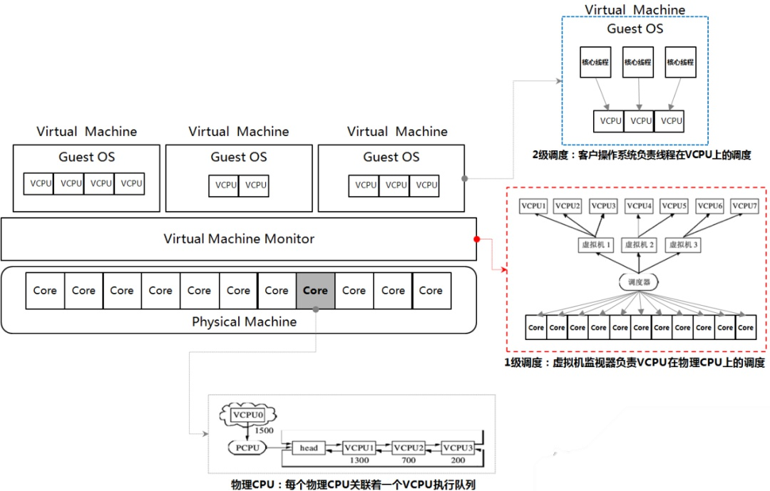
\includegraphics[width=\textwidth]{cloud-cpu-virtualization.png}
        \end{center}
    \end{figure}
\end{remark}



\subsection{CPU全虚拟化}
主要采用优先级压缩技术(\term{Ring Compression})和二进制代码翻译技术Binary Translation) . 优先级压缩技术让VMM和Guest运行在不同的特权级下。 

对X86架构而言,即VMM运行在最高特权级别Ring 0下, Guest OS运行在Ring 1下,用户应用运行在Ring 3下。 因此Guest OS的核心指令\textbf{无法直接下达到计算机系统硬件执行},而是需要经过VMM的\textbf{捕获}和\textbf{模拟}执行(部分难以虚拟化的指令需要通过\term{Binary Translation}技术进行转换) . 

\begin{figure}[htbp]
    \begin{center}
        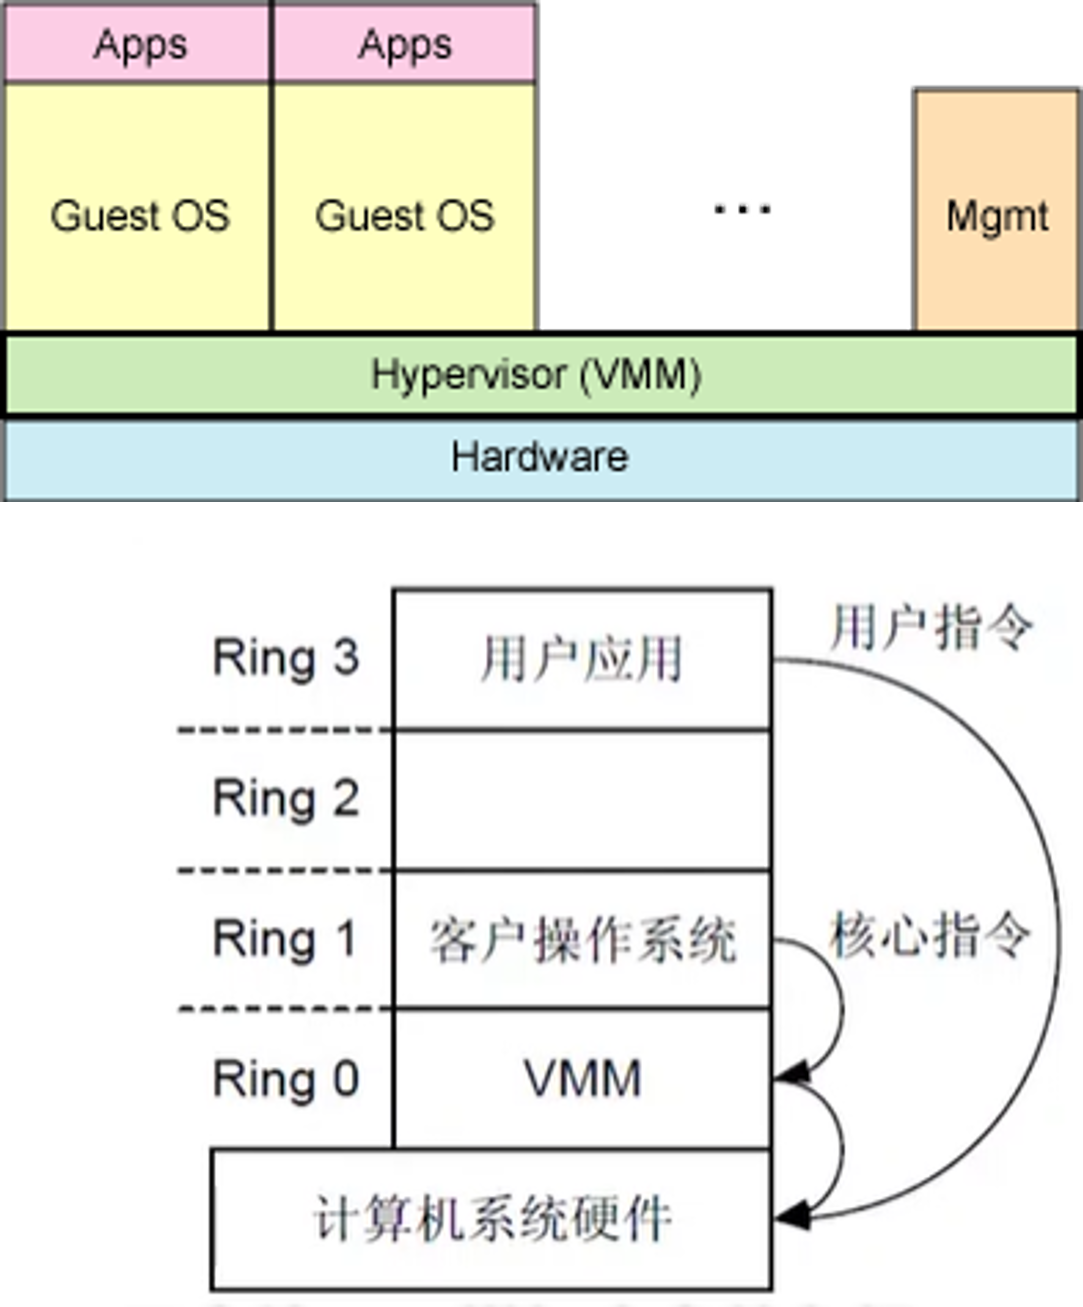
\includegraphics[]{cloud-cpu-full-virtualization.png}
    \end{center}
\end{figure}

\subsection{CPU半虚拟化}
    
主要采用\term{Hypercall}技术。 

\textbf{Guest OS的部分代码被改变},从而使Guest OS会将和特权指令相关的操作都转换为发给VMM的Hypercall (超级调用) ,由VMM继续进行处理。 而Hypercall支持的批处理和异步这两种优化方式,使得通过Hypercall能得到近似于物理机的速度。 

\begin{figure}[htbp]
    \begin{center}
        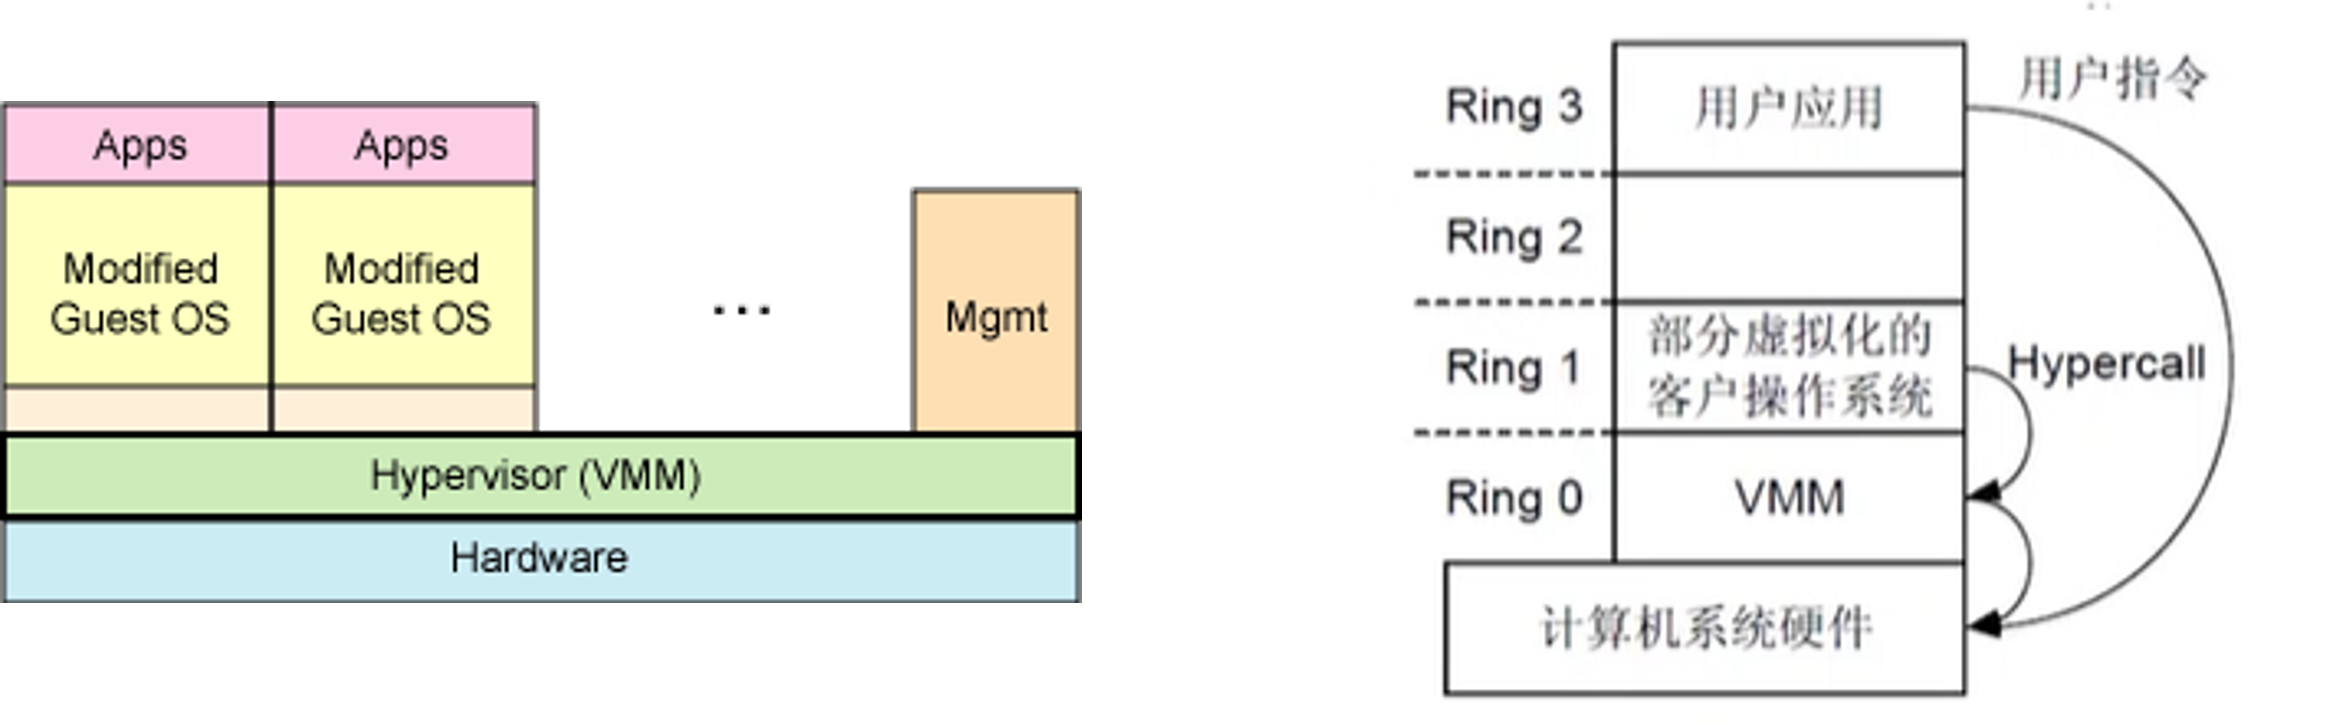
\includegraphics[width=\textwidth]{cloud-cpu-para-virtualization.png}
    \end{center}
\end{figure}

\subsection{CPU硬件辅助虚拟化技术}

目前主要有Intel的\term{VT-x}和AMD的\term{AMD-V}这两种技术。 

其核心思想都是通过引入新的指令和运行模式,使VMM和Guest OS分别运行在不同模式(\term{Root模式}和非ROOT模式)下,且Guest OS运行在Ring 0下。 通常情况下, Guest OS的核心指令可以直接下达到计算机系统硬件执行,而不需要经过VMM,当Guest OS执行到特殊指令的时候,系统会切换到VMM,让VMM来处理特殊指令。 

区分root模式, monitor运行在root模式运行,虚拟机支持非root的ring0,硬件区分来自guest OS指令和host OS指令,核心指令可以直接发送给CPU而无需vmm捕捉

\begin{figure}[htbp]
    \begin{center}
        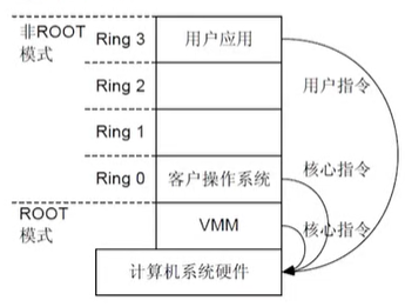
\includegraphics[]{cloud-cpu-assisted-virtualization.png}
    \end{center}
\end{figure}

\subsection{内存虚拟化技术}

内存虚拟化技术的产生:内存虚拟化的产生源于VMM与客户系统在对物理内存的认识上存在冲突,造成物理内存真正拥有者-VMM必须对系统访问的内存进行一定程度上的虚拟化。 

虚拟机的内存映射到真实存储器的顺序: 真实物理内存$\rightarrow$ 其他存储,️超过物理内存时performance下降

$虚拟地址\leftrightarrow^{translation}实际地址$

每个进程看到独立的地址内存空间
假如超过内存空间,需等待其他程序释放

虚拟地址 $\leftrightarrow$ real memory address(虚拟机所看到的虚拟地址) $\leftrightarrow$ physical(物理机看到的虚拟地址)

\subsubsection{内存全虚拟化技术}

通过使用影子页表(Shadow Page Table)实现虚拟化。 

VMM为每个Guest都维护一个影子页表,影子页表维护虚拟地址(VA)到机器地址(MA)的映射关系。 而Guest页表维护VA到客户机物理地址(GPA)的映射关系。 

当VMM捕获到Guest页表的修改后, VMM会查找负责GPA到MA映射的P2M页表或者哈希函数,找到与该GPA对应的MA,再将MA填充到真正在硬件上起作用的影子页表,从而形成VA到MA的映射关系。 而Guest的页表则无需变动。 

page table:虚拟地址$\rightarrow$ 物理地址;有相关技术加速检索

shadow 页表(客户机页表):维护进程的虚拟地址$\rightarrow$ guest os地址(guest physical address,如虚拟机申请的)

p2m页表/哈希函数 GPA地址$\rightarrow$ 机器地址……填充到在硬件上起作用的是影子页表


\begin{figure}[htbp]
    \begin{center}
        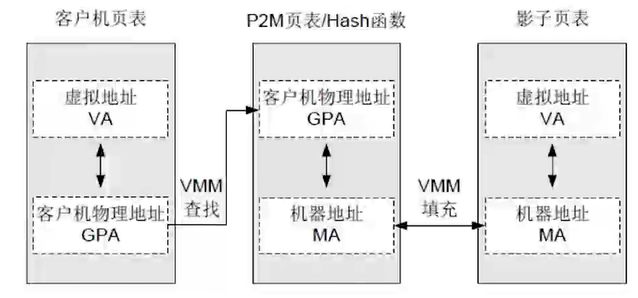
\includegraphics[]{cloud-memory-full-virtualization.png}
    \end{center}
\end{figure}


\subsubsection{内存半虚拟化技术}

通过使用页表写入法实现虚拟化。

Guest OS在创建一个新的页表时,会向VMM注册该页表。 之后在Guest运行的时候, VMM将不断的管理和维护这个表,使Guest上面的程序能直接访问到合适的地址。 

guest os直接向vmm注册, vmm跨层维护页表, virtual address直接翻译成physical address

\subsubsection{内存硬件辅助虚拟化技术}

通过扩展页表EPT (\term{extended page table})实现虚拟化。 

EPT通过使用硬件虚拟化技术,使其能在原有的页表的基础上,增加一个EPT页表,用于记录GPA到MA的映射关系。 VMM预先把EPT页表设置到CPU中。 

Guest修改Guest页表,无需VMM干预。 地址转换时, CPU自动查找两张页表完成Guest虚拟地址到机器地址的转换,从而降低整个内存虚拟化所需的开销。 

\begin{figure}[htbp]
    \begin{center}
        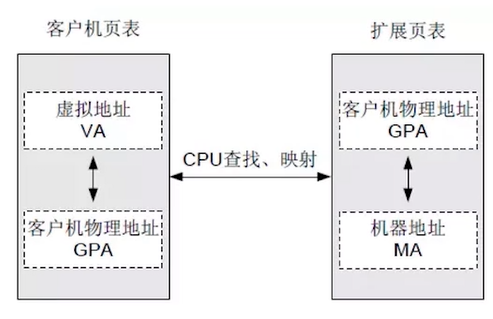
\includegraphics[]{cloud-memory-assisted-virtualization.png}
    \end{center}
\end{figure}

\subsection{I/O虚拟化技术}


\section{常见的虚拟化产品}

\begin{itemize}
    \item Hyper-V虚拟化
    \item Xen虚拟化
    \item Vmware虚拟化
    \item VirtualBox虚拟化
    \item KVM虚拟化
    \item Docker虚拟化
\end{itemize}


\section{容器}

\begin{definition}[容器]
    利用一个开源的容器引擎,让开发者可以打包他们的应用以及依赖包到一个可移植的镜像中,然后发布到任一Linux或Windows机器上,也可以实现虚拟化。 
\end{definition}

\begin{definition}[镜像]
    可执行的独立软件包,包含软件运行的内容:代码,运行时环境,系统工具,系统库和设置。 
\end{definition}

\begin{definition}[Docker]
    基于容器技术的\textbf{轻量级}虚拟化解决方案。 Docker是容器引擎,把Linux的cgroup、namespace等容器底层技术进行封装抽象,为用户提供了创建和管理容器的便捷界面(包括命令行和API)

\end{definition}

Docker作用:将应用程序与该程序的依赖,打包在一个文件里,运行这个文件,就会生成一个虚拟容器。 程序在这个虚拟容器里运行,就好像在真实的物理机上运行一样。 有了Docker,就不用担心环境问题[将程序和dependency包含在一个image中,使得对于全局配置的依赖解耦(应用和运行环境打包)]. 

\textbf{轻量级}的容器,可以只含有一个APP及其依赖。 base image包含OS等,APP image在base image之上

核心:实现应用与运行环境整体打包以及打包格式统一。 

Docker的好处

\begin{itemize}
    \item 秒级的交付和部署 $\rightarrow$ serverless依赖于轻量级容器技术,执行毫秒级高性能要求任务,重量级容器启动慢,轻量级只包含minimal set,deploy快;不定时的服务需求,需要尽快返回结果$\rightarrow$ 尽快部署, 如搜索服务
    \item 保证环境一致性
    \item 高效的资源利用
    \item 弹性的伸缩
    \item 动态调度迁移成本低
\end{itemize}

一个完整的Docker有以下几部分组成:
客户端(\term{Docker Client})、守护进程(\term{Docker Daemon})、镜像(\term{Docker Image})、容器(\term{Docker Container})、仓库(\term{Docker Registry})

\begin{figure}[htbp]
    \centering
    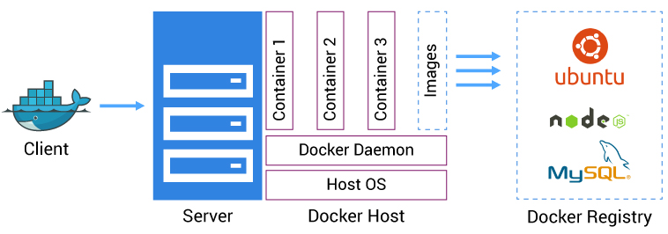
\includegraphics[width=\textwidth]{cloud-docker-architecture.png}
\end{figure}

Docker采用C/S架构,Docker Daemon作为服务端接受来自客户的请求,并处理这些请求(创建、运行、分发容器)。 客户端和服务端既可以运行在一个机器上,也可通过socket或者RESTful API来进行通信。 

Docker daemon一般在宿主主机后台运行,等待来自客户端的消息。 Docker客户端则为用户提供一系列可执行命令,用户用这些命令实现跟Docker daemon交互。 

\begin{figure}[htbp]
    \centering
    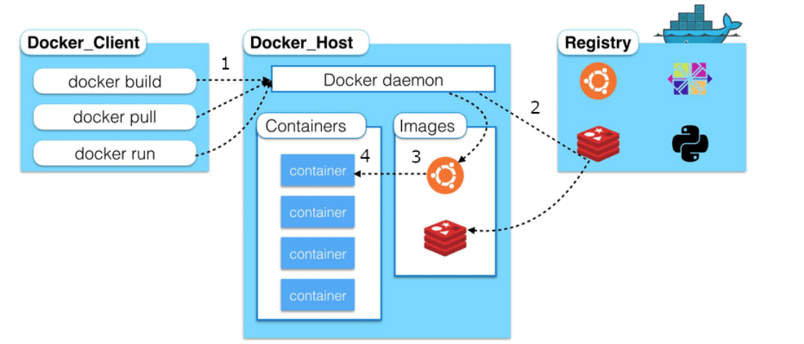
\includegraphics[width=\textwidth]{cloud-docker-architecture-2.png}
\end{figure}

\begin{definition}[Cluster]

\end{definition}

集群:基础运行收费(:只有运行时才能autoscale)+用户request多收费$\rightarrow$ 适用于中小企业

\begin{example}
    10 tasks:查询的数据库、代码等需先存入️集群中, 
当有新请求时,️自动部署新容器
\end{example}

集群由k8s管理,效率高; 有弹性; live migration成本低

\section{虚拟机与容器的对比}


\begin{figure}[htbp]
    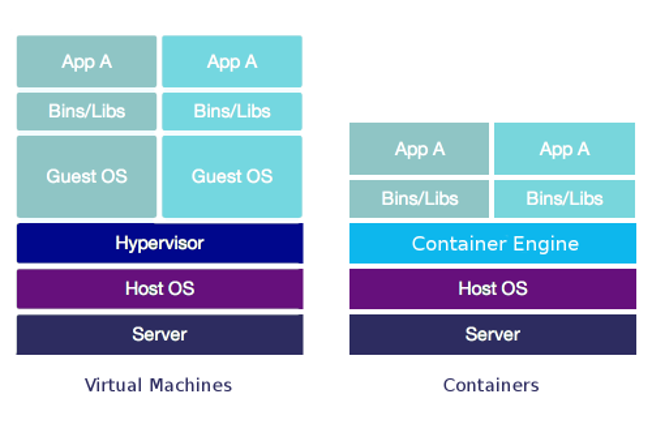
\includegraphics[width=\textwidth]{cloud-vmware-container-architecture.png}
\end{figure}

\begin{figure}[htbp]
    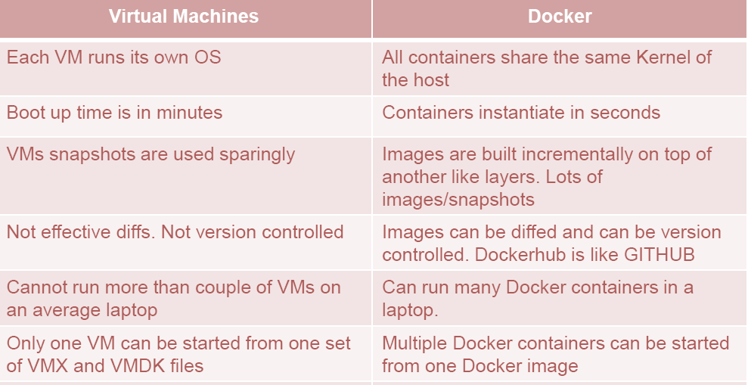
\includegraphics[width=\textwidth]{cloud-comparison-vmware-docker.png}
\end{figure}

\section{MapReduce, 并行}

\term{concurrent 并行}:同时进行

\term{(分时)并发}:2个任务同时发生,看似同时运行,但未必同时进行

\subsection{调度}

不同任务之间、不同io/网络等

MapReduce$\rightarrow$ Hadoop ,spark $\rightarrow$ spark的调度